\documentclass[space,handout]{ximera}

\title{Drug Decay, Part 2}

\begin{document}
\begin{abstract}
Here we continue to investigate various models for the ``behavior'' of drugs in our bodies.  
\end{abstract}
\maketitle

\section{Reminder}
Pharmacokinetics is the study of the behavior of drugs and other substances administered to living organisms.  
The well-established general model for 
the elimination of a given drug from the body of a given human being is given by the differential equation 
$$y'(t)=-\frac{ky(t)}{A+y(t)}$$
where $y(0)$ is the initial concentration in, say, milligrams per liter, and $y(t)$ is the concentration at time $t$.  The constants $k$ and $A$ depend, of course, on the particular drug and the particular human being. 


\section{Background for Today's Activity}
For most pharmaceuticals, $y(t)$ is usually very small in comparison
to $A$.  So again, we replace the general model with a simpler model
$y'(t)=-\frac{k}{A}y(t)$, where $y(0)$ is the concentration at time
$t=0$.  But many pharmaceuticals are taken not once but at regular
intervals over time.

When a drug is effective in the body, the concentration of the drug is
said to be at a \textbf{therapeutic level}.  At such a level, the
\textbf{maintenance dose} is the amount to be taken, say daily, to
offset the amount ``cleared'' by, e.g., the kidneys and the liver in
that time interval.

\section{The Discrete Case}
Before we use this model to describe how such drugs behave
continuously over time, we investigate the \textbf{discrete case}
where we consider the concentration in the body immediately before and
immediately after each dose.  The following example is adapted from
\href{http://en.wikipedia.org/wiki/Loading_dose}{Wikipedia}.

\newpage
\begin{question}
  Suppose the hypothetical drug foosporin has a long lifetime in the
  body, and only ten percent of it is cleared from the blood each day
  by the liver and kidneys. Suppose also that the drug works best when
  the total amount in the body is exactly one gram. Fill in the table
  below where the maintenance dose is $100$ mg. \textbf{Round your answers to the
  nearest milligram.}
  \[
  \begin{array}{|c|c|c|}
    \hline
    \text{Day} & \text{Dose} & \text{Remaining} \\ \hline
    0  & 100\,\text{mg} & 100\,\text{mg} \\ \hline
    1  & 100\,\text{mg} & \answer[tolerance=0]{190}\,\text{mg}\\ \hline
    2  & 100\,\text{mg} & \answer[tolerance=0]{271}\,\text{mg}\\ \hline
    3  & 100\,\text{mg} & \answer[tolerance=0]{344}\,\text{mg}\\ \hline
    4  & 100\,\text{mg} & \answer[tolerance=1]{409.5}\,\text{mg}\\ \hline
  \end{array}
  \]
\end{question}

\begin{question}
Now suppose a patient started taking $100$ mg of foosporin every day.
Make a table showing how the amount of foosporin in the body changes
over time.  How many days will it take to reach the therapeutic level?
\textbf{Answer in a whole number of days}
\[
\answer[tolerance=1]{343}\qquad\text{days.}
\]
\begin{hint}
  You can express the total amount of the drug after $n$ days in the
  body with the following expression:
  \[
  100 + 0.9\cdot 100 + 0.9^2 \cdot 100 + 0.9^3 \cdot 100 +\cdots + 0.9^n \cdot 100
  \]
\end{hint}
\begin{hint}
  You can find a closed-form expression by setting:
  \[
  S(n)= 100 + 0.9\cdot 100 + 0.9^2 \cdot 100 + 0.9^3 \cdot 100 +\cdots + 0.9^n \cdot 100,
  \]
  computing $S(n) - 0.9 S(n)$ and solving for $S(n)$.
\end{hint}
\end{question}


\begin{question}
When a drug takes a long time to reach the therapeutic level, a doctor
might prescribe a \textbf{loading dose} to be taken on the first day
to get the drug's concentration immediately up to that level. Which
graph below best shows the amount of a drug in your system, assuming
an initial loading dose and a regular maintenance dose?
\begin{image}
  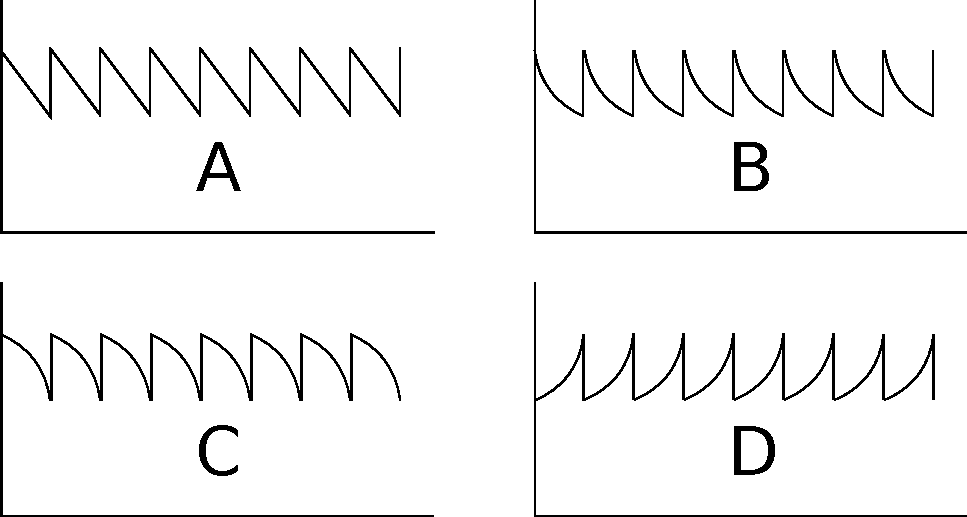
\includegraphics{plots.pdf}
\end{image}
\begin{multipleChoice}
  \choice{A}
  \choice[correct]{B}
  \choice{C}
  \choice{D}
\end{multipleChoice}
\end{question}


%% \begin{question}
%% When a drug takes a long time to reach the theraputic level, a doctor
%% might prescribe a \textbf{loading dose} to be taken on the first day
%% to get the drug's concentration immediately up to that level.  What
%% should the loading dose be?  Make a new table showing how the amount
%% of foosporin in the body changes over time.
%% \begin{freeResponse}
%% \end{freeResponse}
%% \end{question}

%% \section{The Continuous Case}
%% Now we consider the continuous case.  
%% \begin{question}
%% Draw a graph that shows how foospirin concentration varies over one week after an initial \textbf{loading dose}.  Assume that the doses are absorbed immediately into the bloodstream.  
%% \begin{freeResponse}
%% \end{freeResponse}
%% \end{question}

%% \begin{question}
%% Draw a graph that shows how foospirin concentration varies over one week, this time without a loading dose.  Again assume that the doses are absorbed immediately into the bloodstream.  
%% \begin{freeResponse}
%% \end{freeResponse}
%% \end{question}

%% \newpage
%% \begin{question}
%% Most drugs have a \textbf{theraputic window}, which is a range of concentrations, below which the drug is not effective and above which the drug is toxic.  Draw a graph of a drug that requires three doses to reach the theraputic level.  
%% \begin{freeResponse}
%% \end{freeResponse}
%% \end{question}

%% \begin{question}
%% Write down some additional questions about this context.       
%% \begin{freeResponse}
%% \end{freeResponse}
%% \end{question}

\end{document}

